\chapter{Introduction}
\label{chap:introduction}

\todo{I do all my work in Haskell but I never mention Haskell anywhere... I need to remedy this}

\begin{LaTeXdescription}
    \item What is a general purpose language?
\end{LaTeXdescription}

The answer to this question can be summarized as "A computer language that is broadly applicable across application
domains, and lacks specialized features for a particular domain".

Does the answer imply that it is completely arbitrary, which language we should choose for a specific project? We should be
able to implement arbitrary software in a general-purpose language.

The answer is surely no. A language can be general purpose in that any software could be implemented in it, but
actually excels at writing software for a \textit{specific domain}. As an example, consider Erlang \cite{DBLP:conf/hopl/Armstrong07}. It is general purpose,
but really excels at writing programs that need to be distributed and scalable. In a way, Erlang is both a general-purpose
language and a domain-specific language.

Another example of such a language is C. C is used to implement systems for all kinds of domains, but it excels when you
need to write code that reasons about the hardware\todo{rephrase} it runs on. This is one of the reasons why C is so popular; the proximity
to the hardware allows the programmer to take advantage of system resources and write fast, efficient code.

A domain-specific language \cite{DBLP:journals/csur/Hudak96} is domain-specific because it has language primitives that allow a programmer to concisely
express behavior that is common in a specific domain. In Erlang, it is very easy to create concurrent processes that perform
tasks, where the runtime system of Erlang makes sure to use available cores on the machine it executes on. The same behavior
can be expressed in C, but since C lacks abstractions for expressing this, a lot more code has to be written to achieve the
same behavior. More code means more bugs, higher maintenance costs, and perhaps a larger software team. These statements are
highly relevant for the work described in this thesis, as the argument of this thesis is that the line between a general-purpose
and domain-specific languages can be very blurry, and it is important to choose the \textit{right tool for the job}.

% To emphasize the importance of this, the following two sections will present two different application domains. Examples of simple
% applications will be given for each domain, which will be used to illustrate that the lack of domain-specific abstractions lead
% to the implementation becoming more complicated than necessary.

The remainder of the thesis will detail my research on domain-specific languages. The thesis begins by motivating
why domain-specific languages are needed. We then cover some important background topics. After that, the
two papers that make up this thesis follow.

\section{Time}

Consider a simple program
that flashes an LED at a fixed frequency. This program is the "Hello world!" of microcontroller programming, and is often distributed
as an example application with operating systems for microcontrollers. It illustrates how to perform
periodic tasks that do IO. The desired output should vary over time as illustrated in figure \ref{graphics:correct-frequency}.

\begin{figure}
    \centering
    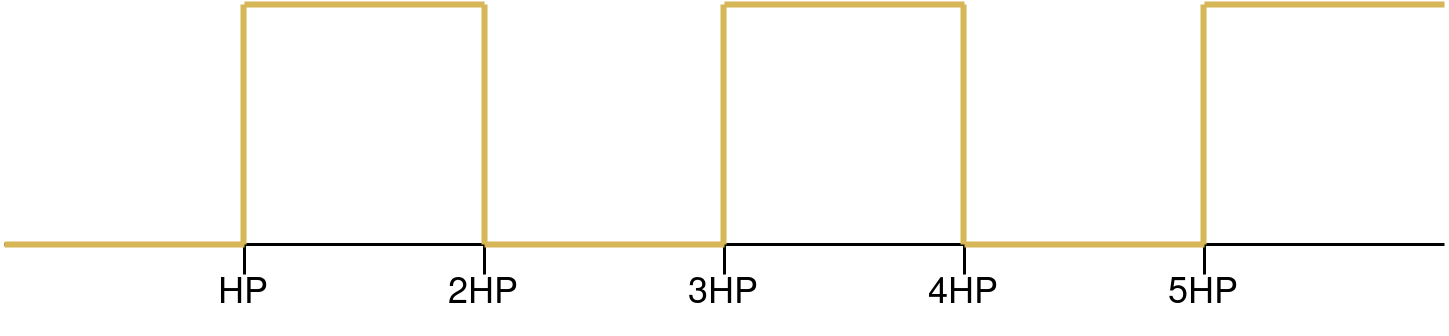
\includegraphics[scale=0.2]{graphics/correct-frequency.png}
    \caption{The signal in the diagram changes state with the desired frequency, where each change occurs at the half-period points.}
    \label{graphics:correct-frequency}
\end{figure}

A pseudo-code variant of the program, as it is often illustrated, is shown below.

\begin{verbatim}
    void main() {
        while(1) {
            toggle_led(the_led);
            sleep(half_period);
        }
    }
\end{verbatim}

An equivalent version of the same program could use alarms and callbacks to specify what should happen at what time. Such
a version of the program appears below.
\begin{verbatim}
    void toggle() {
        toggle_led(the_led);
        set_alarm(half_period, &toggle);
    }

    void main() {
        configure_timer();
        set_alarm(half_period, &toggle);
    }
\end{verbatim}

The main function above configures some timer and sets an alarm that, when the alarm goes off, will trigger an invocation of
the \code{toggle} function. The \code{toggle} function flips the current value of the LED and then sets a new alarm.
While the code is very simple and seems to implement the desired semantics, it is buggy! The frequency will not be
the one we want. When the alarm goes off and the function is invoked, the function performs some operations before the next
alarm is set. If we call the time it takes to perform the operations $\delta_{op}$ and the half period $hp$, the times the
alarm goes off are $$0, \delta_{op} + hp, 2(\delta_{op} + hp), 3(\delta_{op} + hp), 4(\delta_{op} + hp), ...$$

This sequence illustrates that, as time progresses, the frequency drifts further and further away from the target. See
figure \ref{graphics:drift}.

\begin{figure}
    \centering
    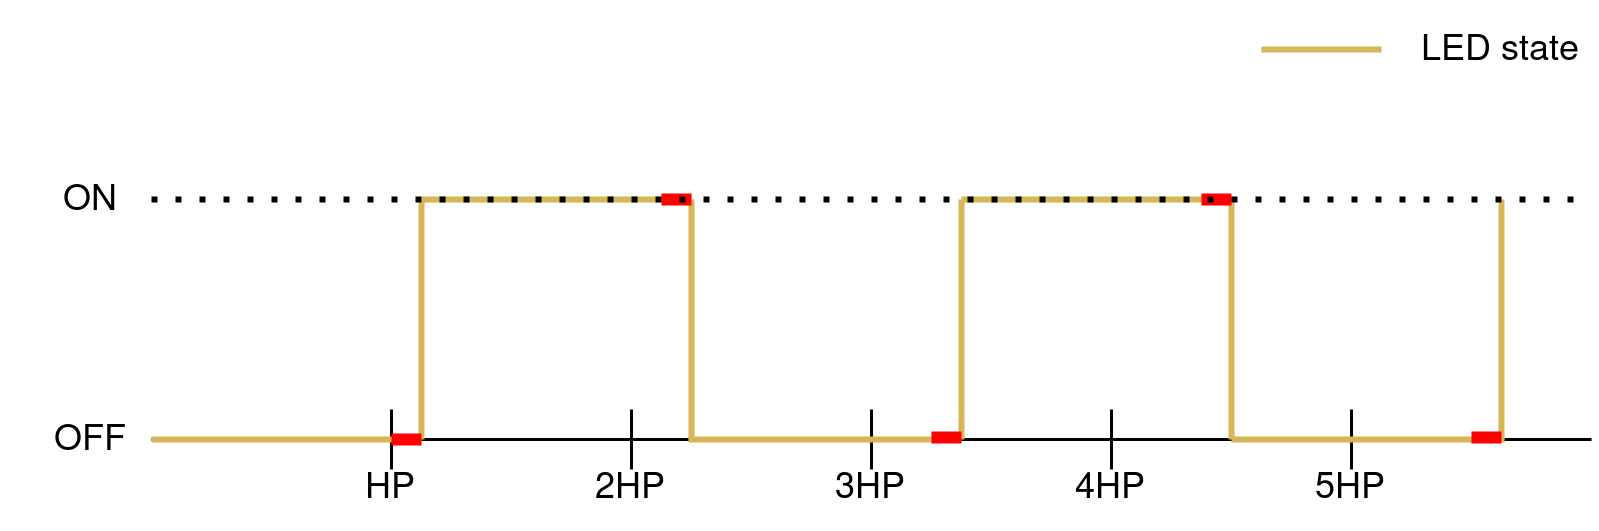
\includegraphics[scale=0.2]{graphics/drift.png}
    \caption{The diagram illustrates where the half-period points are, and where the changes signal occur. The red
    segments illustrate the time $\delta_{op}$ takes. The additions of $\delta_{op}$ lead to the signal drifting
    further and further away from the half-period points.}
    \label{graphics:drift}
\end{figure}

Let us try to fix our program to allow for the time it takes to perform the operations.
As soon as \code{toggle} is invoked, we query the system for the current time. The next time we set
the alarm we configure the alarm to go off relative to the previously sampled time.

\begin{verbatim}
    time current;

    void toggle() {
        current = current_time();
        toggle_led(the_led);
        set_alarm_relative_to(current, half_period, &toggle);
    }

    void main() {
        configure_timer();
        current = current_time();
        set_alarm_relative_to(current, half_period, &toggle);
    }
\end{verbatim}

Even with the alarm set relative to when the process last woke up, the frequency suffers from drift. An oscilloscope
will report that the drift is smaller than before, but still present. This remaining source of drift is a bit
trickier to account for.

When the actual hardware clock reaches the point where an alarm should be raised, it takes some time for the
operating system to locate the \code{toggle} function and invoke it. To account for this delay, we can choose to
set alarms not relative to when \code{toggle} was last invoked, but rather relative to when \code{toggle}
\textit{was supposed} to have been invoked. We do this by implementing a logical clock that is incremented to reflect
what the time of the system should be.

\begin{verbatim}
    time current;

    void toggle() {
        current = current + half_period;
        toggle_led(the_led);
        set_alarm_absolute(current + half_period, &toggle);
    }

    void main() {
        configure_timer();
        current = 0;
        set_alarm_absolute(current + half_period, &toggle);
    }
\end{verbatim}

The program now maintains a global variable that tracks the current time. An absolute alarm is set that will go off at
time \code{current + half\_period}, regardless of what time it is when the alarm is set. The next time \code{toggle}
is invoked, it is assumed that time has progressed to \code{current + half\_period}, and the logical time is updated
to reflect this. If the system time is queried at this point, it will show that the current time is 
\code{current + half\_period +} $\delta_{lookup}$, where $\delta_{lookup}$ is the amount of time it takes for the
\code{toggle} function to be found and invoked.

Executing this program will yield a signal of the correct frequency. Since the delay for the system to look up and
invoke the callback ($\delta_{lookup}$) is still there, there is a small phase error (the size of which is equal to
$\delta_{lookup}$), but the frequency is still stable and correct. This signal is illustrated in figure \ref{graphics:phase-error}

\begin{figure}
    \centering
    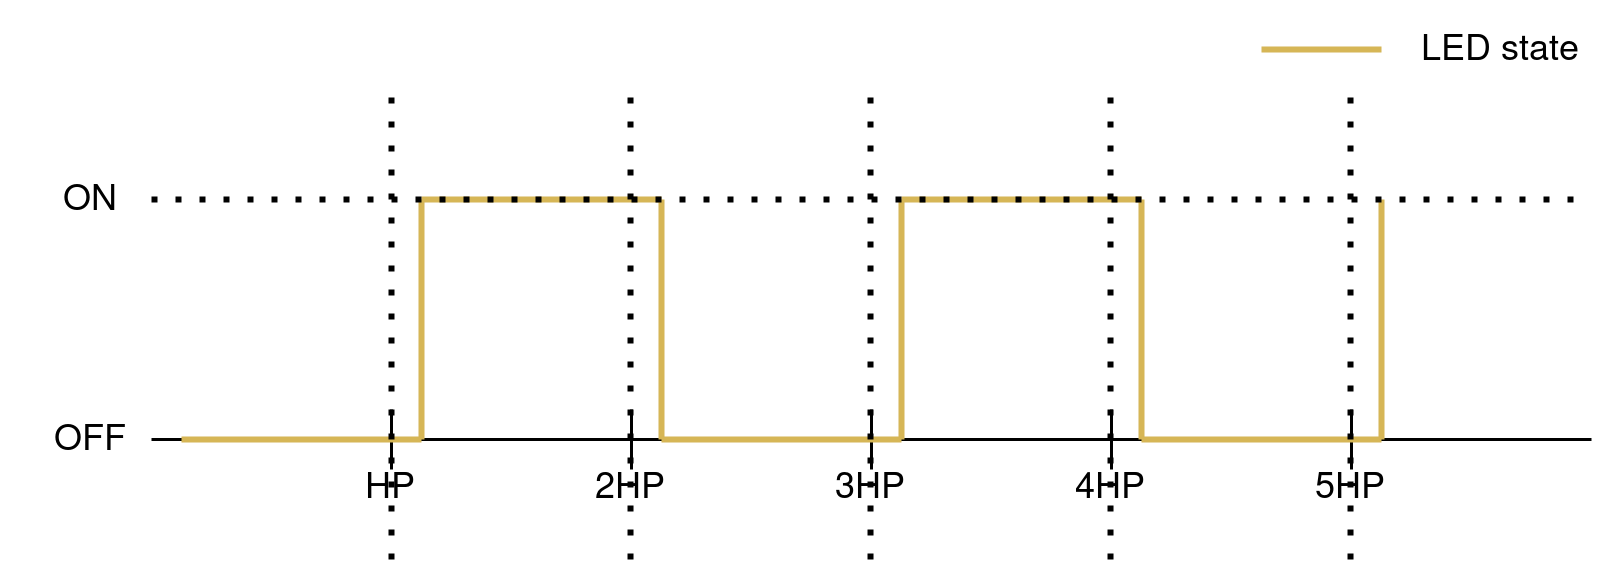
\includegraphics[scale=0.2]{graphics/phase-error.png}
    \caption{The diagram illustrates the correct frequency as generated by the final version of our program. There is
    a small phase error, indicated by the dotted lines. The dotted lines denote the actual half-period points, but
    the distance from the signal transition to the half-period points remains constant. The distance is of duration
    $\delta_{lookup}$.}
    \label{graphics:phase-error}
\end{figure}

While the initial program seemed intuitively reasonable, it was actually erroneous. The final version is
correct (up to the phase error), but is substantially more complicated. While the pseudo-code might look short and
simple, still, we now have a program that maintains a logical time and sets absolute deadlines, something that is easy
to get wrong.

The extra complication is a result of the primitive timing API in a language such as this. Querying the system for the current
time and setting alarms is a very coarse API. The fact that the system does not assist the developer with accounting for
systematic delays and the time it takes to perform computations makes the whole business of reasoning about deadlines much more difficult.

\textcolor{red}{tie this back to DSLs // John's comment}

\section{Confidential Computing}

A second non-trivial application domain is that of confidential computing. Confidential computing is the act of protecting
\textit{data in use}.
Data always exists in one of three states. It can exist as \textit{data in motion}, as \textit{data at rest}, or as
\textit{data in use}. Data in motion is data that is moving from one part of the system to another, e.g. via TCP, while data at rest
is data that is being stored in persistent memory. Both of these kinds of data can be protected via e.g. encryption.
Encryption is enough to guarantee confidentiality in these cases if you trust your encryption scheme.

Data in use, however, is a bit different. To perform any meaningful operations on data, it has to be loaded in from
persistent storage. Consider the pseudo-code below

\begin{verbatim}
    (int, int) process_data(int x, int y) {
        return (x+2, x*y);
    }

    void server(key) {
        req          = await_request();
        (ct1, ct2)   = load_data(req);
        (pt1, pt2)   = (decrypt(ct1, key), decrypt(ct2, key));
        (r1,r2)      = process_data(pt1, pt2);
        (nct1, nct2) = (encrypt(r1, key), encrypt(r2, key));
        store((nct1, nct2));
    }
\end{verbatim}

The code consists of two parts. One part is the \code{server} function, which deals with communication and parsing of
incoming requests. The second part is actual application logic, which is very simple in this example. \code{server}
receives a request that indicates which confidential data should be loaded from the data storage. The data is decrypted before
it is handed off to the \code{process\_data} procedure, after which the result is encrypted and written back to data storage.

One problem with this code is that the data is decrypted before it is operated on. The result of this is that it exists in
plaintext form in the RAM of the machine the code is running on, and an attacker running on the same machine, such as a
compromised OS, might leak this data. This is illustrated
in figure \ref{graphics:unsafe-data-in-use}.

\begin{figure}
    \centering
    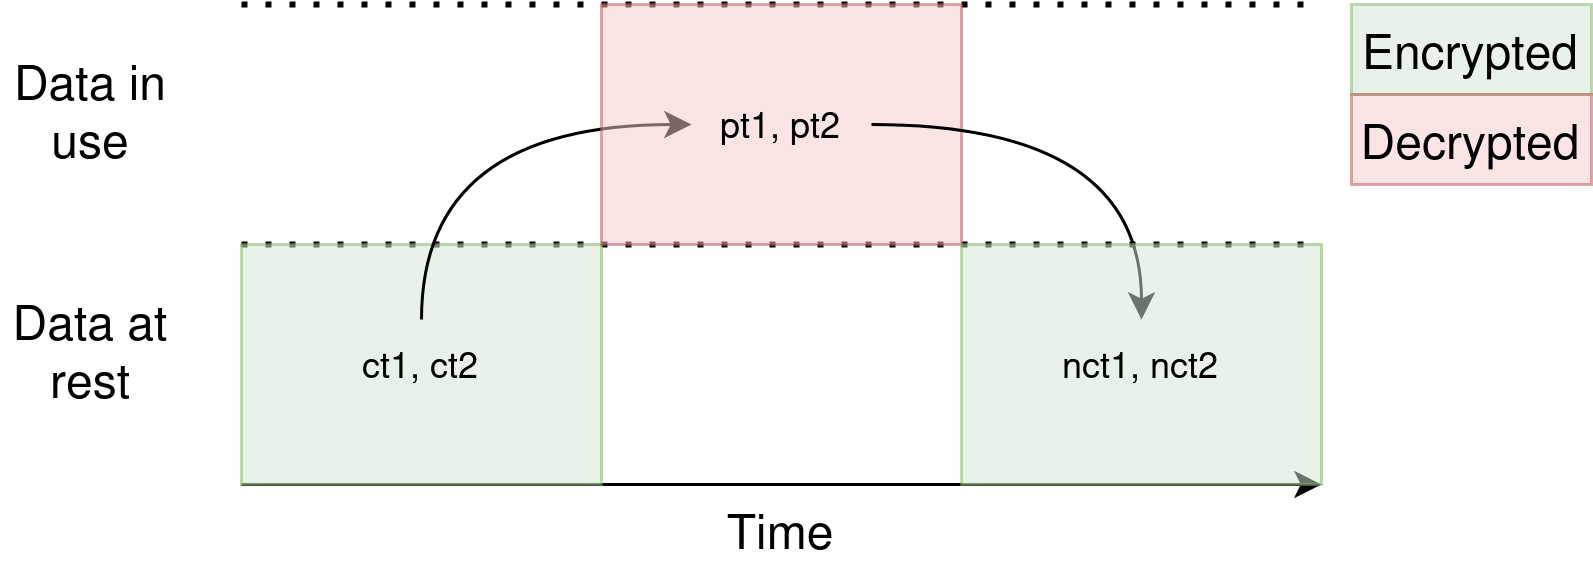
\includegraphics[scale=0.2]{graphics/unsafe-data-in-use.png}
    \caption{The diagram illustrates that while the data is at rest, it exists in encrypted form. When the data
    is operated on, it is loaded from the data storage and decrypted (as indicated by the red color), before the result is encrypted and
    written back to the data storage.}
    \label{graphics:unsafe-data-in-use}
\end{figure}

One technique for mitigating this is to apply homomorphic encryption\cite{DBLP:conf/stoc/Gentry09}. Homomorphic encryption is a form of encryption where
operations can be performed on the encrypted data without decrypting it, such that the decrypted result is the correct one.

\begin{verbatim}
    (int, int) process_data(int x, int y, Key key) {
        two   = encrypt(2, key);
        left  = homo_add(x, two, key);
        right = homo_mul(x,y, key);
        return (left, right);
    }

    server(key) {
        req          = await_request();
        (ct1, ct2)   = load_data(req);
        (r1,r2)      = process_data(data1, data2, key);
        store((r1,r2))
    }
\end{verbatim}

\begin{figure}
    \centering
    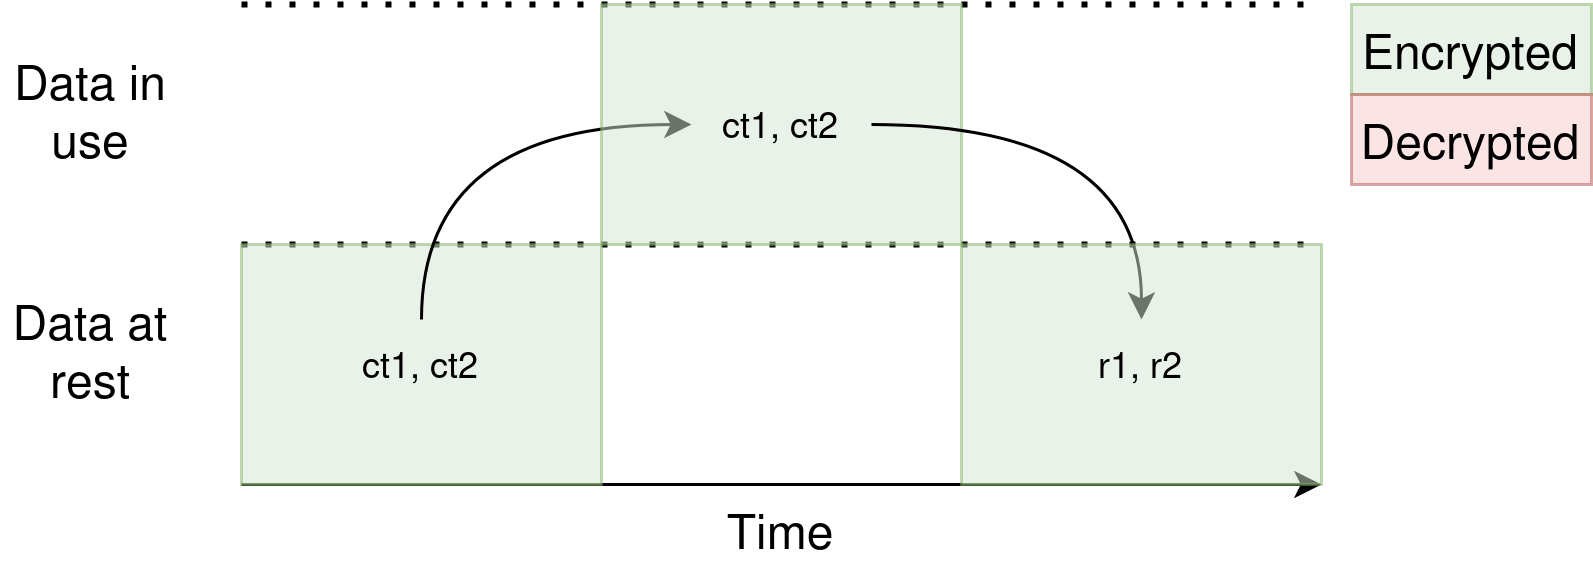
\includegraphics[scale=0.2]{graphics/safe-data-in-use.png}
    \caption{By applying homomorphic encryption, the data does not need to be decrypted before it is processed. The result
    of the computation is already encrypted, and is written back to the disk directly.}
    \label{graphics:safe-data-in-use}
\end{figure}

\textcolor{red}{FIXME: the key is still in RAM, need to say something about this}
In the above code, the data is never decrypted, as illustrated in figure \ref{graphics:safe-data-in-use}. Even if the OS is compromised, and the contents of the RAM leaked, the
data is not leaked in plaintext form. A downside of this approach is that the procedure that processes the data is now
much more complicated. It needs to apply special operations in place of ordinary ones. This obfuscates the code and
adds extra complexity. In the presence of a bug, it could also be harder to debug this code. While the example program
above still looks fairly simple, it does not scale very well.

Ideally, the program above would be described only in terms of the application logic. Encryption is an orthogonal part of
the application that just "needs to happen", and is not necessarily part of the application logic.

\todo{The time section ends with a solution to the described problem, whereas I don't do that here. Perhaps I should do this.}

\section{Background}

Below follows some sections that describe core topics that are relevant to my thesis.
\textcolor{red}{Why are they important? // John}

\subsection{Synchronous Languages}

\textcolor{red}{
TODO mentions reactive programming, that synchronous languages give a nice framework for writing programs that
react to events. Dataflow programming, say what streams are, etc. Will expand a lot on this section}

The class of synchronous languages is languages where execution unfolds as a sequence of conceptually zero-time instants. Computations
take place within an instant, and logical time does not advance until the next instance. A consequence of this is that all
computation is assumed to happen instantaneously, which leaves a model of execution where time only advances at specific
points. Such a model allows a developer to more easily reason about the temporal behavior of their program.
While this doesn't correspond to how execution actually happens (where computations are not instantaneous), a sufficiently
fast implementation will meet all deadlines and expose real-time properties.

The seminal work on synchronous languages encompasses the languages Lustre\cite{DBLP:conf/popl/CaspiPHP87}, Esterel
\cite{DBLP:journals/scp/BerryG92}, and Signal\cite{DBLP:journals/scp/BenvenisteGJ91}. The language abstractions
are not entirely unfamiliar -- e.g. Lustre allows a developer to declare nodes. A node may receive input streams and produce
an output stream, as well as maintain a state between instants. A stream always has a value. Nodes can compose with other
nodes, where the output stream of one node becomes the input stream of another node.

Esterel exposes even more familiar abstractions in the form of threads. A thread may communicate with other threads by the
use of signals. When a signal arrives it might wake up a thread that is blocking, enabling it to resume execution.

Common to these languages is that a compiler takes a program and compiles everything down to a single step-function, that
when invoked receives input for the entire program and recomputes the new outputs. During runtime, the program is governed
by a global clock, and the step function is invoked when the clock ticks. This is illustrated in figure \ref{graphics:global-clock}.

\begin{figure}
    \centering
    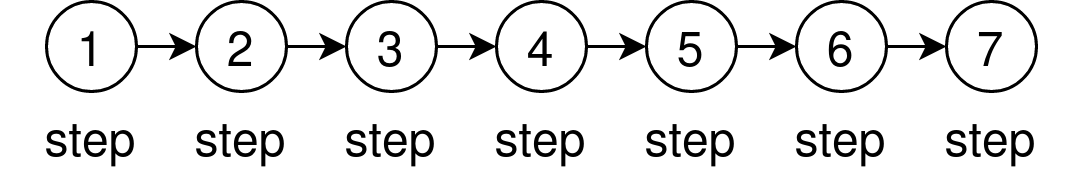
\includegraphics[scale=0.2]{graphics/clock-governed.png}
    \caption{Upon each tick of the global clock, the step function is invoked, and the whole program
    is evaluated for the instant denoted by the index of the tick.}
    \label{graphics:global-clock}
\end{figure}

Despite the languages being tailored to writing programs with temporal behaviors, it is not possible to reason
about time directly. A node can reason about a future instant in relation to previous instants but does not have
a way to instruct the system to do something at a certain time. In Lustre, the global system clock can be seen
as a stream of successive instants, where the time between instants is known. It is then up to the implementation to supply
the specified stream with the correct period.

Synchronous languages have been used successfully to implement real-time, mission-critical applications. E.g
Copilot\cite{DBLP:conf/rv/PikeGMN10} is used to write hardware monitors for avionic systems. This is made possible by generating
the step function such that it runs in constant time.

While synchronous languages have been successfully used for many decades by this point, there are some shortcomings.
The way that a program is governed by a global clock that continually invokes the step function does not lend itself nicely to
certain application domains. If your program reaches a point where it will not do anything for 2 seconds, and we have a global
clock that ticks every microsecond, then we will invoke the step function 2000 times despite the outputs never changing.
An obvious optimization here is to implement a runtime that recognizes that nothing will happen for this period of time,
which allows the runtime to go into a low-power mode to conserve energy. Work on this has materialized as the
\textit{Sparse Synchronous Model} \cite{DBLP:conf/fdl/EdwardsH20}, which has been shown to be appropriate for such
application domains. This sparsity is illustrated in figure \ref{graphics:sparse-clock}.

\begin{figure}
    \centering
    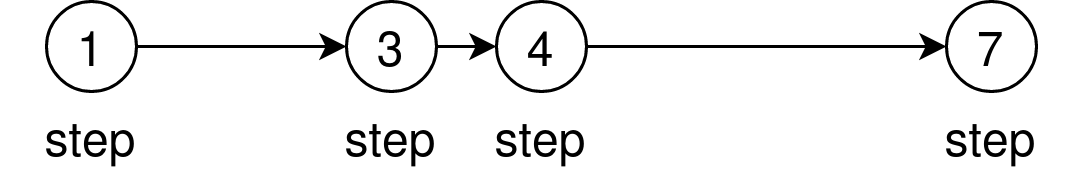
\includegraphics[scale=0.2]{graphics/sparse-clock.png}
    \caption{In contrast to the synchronous model, the sparse synchronous model allows the runtime system to
    detect that no computation should take place for some time. Not having to invoke the step function
    leaves the system open to perform other tasks, and if none exist, to sleep and conserve energy.}
    \label{graphics:sparse-clock}
\end{figure}

\subsection{Embedded Domain-Specific Languages}

Implementing a programming language requires considerable engineering effort. At the very least, a parser and interpreter
has to be implemented. More than often there are many more phases involved, such as type checking, renaming, etc.

A lot of engineering effort can be spared by implementing a language as an embedded language. An embedded language is implemented in another language, called the host language, as a library. By embedding a language in a host language, many phases from the host
compiler can be directly inherited by the new language, such as the parser, type checker, code generator, etc.

The host language becomes a very powerful meta-language for meta-programming in the embedded language. This is a
result of the two runtimes -- the runtime of the host language and the runtime of the embedded language. During host language
runtime, programs in the embedded language can be combined, manipulated, and optimized to produce other programs.

As an example, consider a fragment of the Scoria language, embedded in Haskell.

\begin{verbatim}
    wait :: [Ref] -> SSM ()
    fork :: [SSM ()]
    procedure -- synthesize procedure
\end{verbatim}

The \code{wait} procedure takes a list of references as input, and blocks until \textit{either} of them has received an update.
\code{fork} spawns any number of concurrent child processes, and blocks until \textit{all} of them have terminated.
\code{procedure} takes a Haskell function body and turns the function into a procedure in the embedded language.

Something missing from Scoria, but that we can implement with the help of the host language, is a variant of the
\code{wait} procedure that blocks until \textit{all} references have received updates.

\begin{verbatim}
    waitSingle :: Ref -> SSM ()
    waitSingle ref = procedure $ do
        wait [ref]
    
    waitAll :: [Ref] -> SSM ()
    waitAll refs = fork $ map waitSingle refs
\end{verbatim}

\code{waitSingle} creates an embedded Scoria procedure which, during Scoria runtime, waits for a
single reference to receive an update. \code{waitAll} is a Haskell function which, during Haskell runtime, takes a list of
references and produces a \code{fork} statement that, during Scoria runtime, produces child processes that each
invoke \code{waitSingle} with one of the references. Since \code{fork} does not terminate until all child processes
terminate, \code{waitAll} will not terminate until all references received updates. The code exploits the fact that
\code{waitAll} is executed during Haskell runtime, and expands into code that is executed during Scoria runtime.

The two runtimes also enable principled normalization by evaluation\cite{DBLP:conf/haskell/ValliappanRL21}, by partially evaluating the embedded program during the
host language runtime. \textcolor{red}{TODO write something more here! I am sure I can cite Nachi and say something nice about this. Maybe there
is something fun to say about Feldspar? More fun stuff could be said here!}

While there are many arguments in favor of EDSLs over DSLs, there are also arguments against EDSLs. Two of the bigger arguments
are that the syntax of the embedded language becomes influenced by the host language. A dedicated DSL will employ its own parser,
yielding potential domain-specific syntax that simplifies program development. Another argument is that the choice of host language
might impair programmer efficiency. If an EDSL is embedded in e.g. Haskell, a Haskell developer might be much more efficient
than a C developer, as the Haskell developer knows how to properly take advantage of the host language features.

\textcolor{red}{TODO say more stuff}

\subsection{Information-flow Control}

\todo{rephrase the first part, and slide into IFC in a better way.}
Information-flow control (IFC)\cite{DBLP:series/natosec/HedinS12} ensures that data propagates through a program in such a way that some security policy is
not violated. Values are labeled with a security level, which is then tracked when a value is used to make sure that the
value is not used inappropriately.
A value of one security level can e.g. not influence the result of a value with a lower security level. The property that no data is leaked
in this way is called noninterference.

As a simple example, we describe a language with two security levels, public and secret. We assume that anyone can inspect
a program's public output. The pseudo-code below denotes security levels explicitly in the type signature
of the procedure.

\begin{verbatim}
    public int f(secret int x, public int y) {
        y = x;
        return y;
    }
\end{verbatim}

The above program is ill-formed, as the secret input is assigned to the public output before it is returned. This is an
explicit leakage of information. Implicit leakages are also possible, as in the program below.

\begin{verbatim}
    public bool f(secret bool x, public bool y) {
        if(x) {
            return y;
        } else {
            return (not y);
        }
    }
\end{verbatim}

By inspecting the output we can infer what the secret input was, even though we never directly assign the secret input
to the public variable \code{y}. Note that in both cases, the program would be accepted if we labeled the output as secret.

IFC policies can be enforced statically, dynamically, or through a combination of both. A static policy is checked before
a program is allowed to execute, whereas a dynamic policy is checked at runtime. If the policy is violated, execution
is aborted and an error is raised.

If a value could \textit{never} be downgraded to a lower security level, however, then it would be difficult to write any meaningful program that uses
different security levels. A principled way to release secrets is to explicitly declassify values, giving them a lower
security level.

\begin{verbatim}
secret string stored_pass;

public bool check_password(public string password) {
    secret outcome = compare(stored_pass, password);
    return declassify(outcome);
}
\end{verbatim}

The result of comparing the stored password against the candidate password must be secret, as we had to use the secret stored
password to do the comparison. Before the resulting boolean can be released as a public outcome, we must
\code{declassify} it.

Regardless of whether you use static IFC, or dynamic IFC, or a hybrid variant of IFC, the threat model assumes that the
operating system and runtime system are trusted. In the presence of a compromised operating system, which we assume can
inspect any memory it desires, it does not matter what label a piece of data has. The operating system can inspect and
leak it.

\textcolor{red}{TODO write something more maybe}

\subsection{Trusted Execution Environments}

In an effort to protect data in use, every major hardware vendor is working on support for hardware-enforced trusted
execution environments (TEE). Intel is developing its Intel Software Guard Extensions (Intel SGX)\cite{intelsgx}, Arm is
developing Arm TrustZone\cite{armtz}, AMD is developing different variants such as AMD-SEV\cite{amdsev}, AMD-SME, and
AMD-SEV-SNP, to name just a few. A TEE allocates a contiguous region of memory that contains both secure code and data.
This region of memory can be protected in different ways, with e.g. Intel SGX employing encryption. In the case that the
entire operating system is compromised only encrypted data is visible. Data and code are only decrypted when they move into the
CPU cache. Arm TrustZone instead enforces hardware isolation to separate the memory accessible by untrusted software and
trusted software. \textcolor{red}{TODO read more on this, to verify it}

The programming model for TEEs requires the developer to partition their application into two components. The TEE takes
the role of a server, where the untrusted component makes calls to the enclave. If untrusted code tries to access trusted
data, an error will be raised. This configuration is illustrated in figure \ref{graphics:tee}.

\begin{figure}
    \centering
    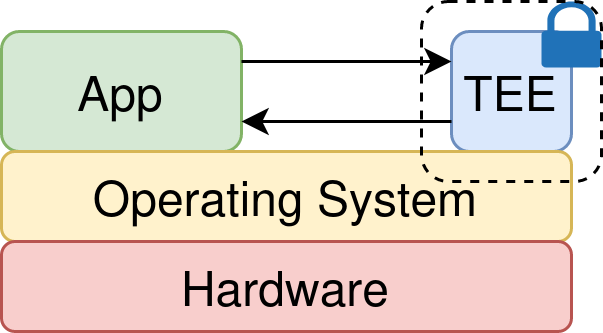
\includegraphics[scale=0.2]{graphics/tee.png}
    \caption{hello}
    \label{graphics:tee}
\end{figure}

While this sounds simple enough, it is in practice quite complicated. Aside from technical complexity
concerning the maintenance of toolchains, actual application development is not trivial. Managing two projects and an
interface between them takes some effort. The TEE application is much more restricted in what it can do, as some
operations are inherently leaky. As an example, applications intended to run on Intel SGX need to be compiled with a
restricted version of the C standard library, where many ordinary functions are missing. This makes it difficult to port
legacy applications to run on Intel SGX, as these applications were written with the assumption that they can access the
whole standard library.

To ease the porting of legacy applications to Intel SGX, projects such as Gramine have emerged (previously called
Graphene \cite{DBLP:conf/usenix/TsaiPV17}). Gramine is a library OS that reintroduces the missing functionality from the
restricted standard library such that any Linux binary can run unmodified.

\section{This Thesis}

The research described in this thesis details my experimentation and exploration of the design and implementation of
DSLs, where I feel that there are unexplored abstractions that warrant experimentation.

In paper 1 I experiment with language design for a language that treats time as a first-class citizen. The programming model
is implemented with support for IO, and the intention is that it should be easy to specify the temporal behavior of a program
without needing to worry about the details of implementation.

In paper 2 we turn Haskell itself into a DSL for writing applications that use secure enclaves. We implement a library that
allows the developer to specify which computations should happen inside an enclave, and which should happen outside. We
then recognize that such a scenario is equivalent to enforcing IFC policies, but in a system where the operating system
does not have to be trusted.

\section{Future work and Conclusions}

Write many interesting future avenues of research!

%%%%%%%%%%%%%%%%%%%%%%%%%%%%%%%%%%%%%%%%%%%%%%%%%%%%%%%%%%%%%%%%%%%%%%%%%%%%%%%%%%%
%%%%%%%%%%%%%%%%%%%%%%%%%%%%%%%%%%%%%%%%%%%%%%%%%%%%%%%%%%%%%%%%%%%%%%%%%%%%%%%%%%%

% \chapter{Summary of Included Papers}
% \label{chap:summary}

% \section{Title of the First Paper}
% \sectionmark{First Paper} % This is in case the title is too long to fit properly in the headings of the following pages

% In this paper we present a method to do something.

% \subsubsection*{Problem}

% Description of what we are trying to solve.

% \vskip 1cm

% Lorem ipsum dolor sit amet, consectetur adipiscing elit, sed do eiusmod tempor incididunt ut labore et dolore magna aliqua. Vel facilisis volutpat est velit egestas dui. Enim ut sem viverra aliquet eget. Lorem sed risus ultricies tristique nulla aliquet. Ultricies mi eget mauris pharetra et ultrices neque. Gravida rutrum quisque non tellus orci ac auctor augue mauris. In fermentum et sollicitudin ac orci phasellus egestas tellus. Orci ac auctor augue mauris augue neque gravida. Facilisi morbi tempus iaculis urna id volutpat lacus laoreet non. Hac habitasse platea dictumst vestibulum. Egestas fringilla phasellus faucibus scelerisque eleifend donec pretium. Auctor elit sed vulputate mi sit amet mauris commodo quis. Vitae nunc sed velit dignissim sodales ut.



% \subsubsection*{Contribution}

% What does the paper do to try to solve the problem?

% \vskip 1cm

% Molestie a iaculis at erat. In vitae turpis massa sed elementum tempus. Tincidunt id aliquet risus feugiat in ante metus. Nunc sed blandit libero volutpat. Pharetra diam sit amet nisl. Eu facilisis sed odio morbi quis commodo odio. Porta lorem mollis aliquam ut porttitor. Metus vulputate eu scelerisque felis imperdiet. Volutpat sed cras ornare arcu dui vivamus arcu felis bibendum. Ultrices mi tempus imperdiet nulla. Tristique sollicitudin nibh sit amet commodo nulla facilisi nullam. Tortor vitae purus faucibus ornare suspendisse sed. Quisque id diam vel quam elementum pulvinar etiam non. Platea dictumst vestibulum rhoncus est pellentesque.


% \subsubsection*{Methodology}

% How is it implemented?

% \vskip 1cm

% Consequat nisl vel pretium lectus quam id. Phasellus egestas tellus rutrum tellus. Id neque aliquam vestibulum morbi blandit cursus risus at ultrices. Est ultricies integer quis auctor elit sed vulputate. Eu consequat ac felis donec et odio pellentesque diam volutpat. Urna id volutpat lacus laoreet non curabitur gravida arcu ac. Scelerisque purus semper eget duis at tellus. Porttitor leo a diam sollicitudin tempor id eu nisl nunc. Mauris nunc congue nisi vitae suscipit tellus mauris. Leo duis ut diam quam nulla porttitor massa id neque. In hendrerit gravida rutrum quisque non. Ornare lectus sit amet est.


% %%%%%%%%%%%%%%%%%%%%%%%%%%%%%%%%%%%%%%%%%%%%%%%%%%%%%%%%%%%%%%%%%%%%%%%%%%%%%%%%%%%
% \clearpage

% \section{Title of the second paper}

% In this paper we present a method to do something else.


% \subsubsection*{Problem}

% Description of what we are trying to solve.

% \vskip 1cm

% Lorem ipsum dolor sit amet, consectetur adipiscing elit, sed do eiusmod tempor incididunt ut labore et dolore magna aliqua. Vel facilisis volutpat est velit egestas dui. Enim ut sem viverra aliquet eget. Lorem sed risus ultricies tristique nulla aliquet. Ultricies mi eget mauris pharetra et ultrices neque. Gravida rutrum quisque non tellus orci ac auctor augue mauris. In fermentum et sollicitudin ac orci phasellus egestas tellus. Orci ac auctor augue mauris augue neque gravida. Facilisi morbi tempus iaculis urna id volutpat lacus laoreet non. Hac habitasse platea dictumst vestibulum. Egestas fringilla phasellus faucibus scelerisque eleifend donec pretium. Auctor elit sed vulputate mi sit amet mauris commodo quis. Vitae nunc sed velit dignissim sodales ut.



% \subsubsection*{Contribution}

% What does the paper do to try to solve the problem?

% \vskip 1cm

% Molestie a iaculis at erat. In vitae turpis massa sed elementum tempus. Tincidunt id aliquet risus feugiat in ante metus. Nunc sed blandit libero volutpat. Pharetra diam sit amet nisl. Eu facilisis sed odio morbi quis commodo odio. Porta lorem mollis aliquam ut porttitor. Metus vulputate eu scelerisque felis imperdiet. Volutpat sed cras ornare arcu dui vivamus arcu felis bibendum. Ultrices mi tempus imperdiet nulla. Tristique sollicitudin nibh sit amet commodo nulla facilisi nullam. Tortor vitae purus faucibus ornare suspendisse sed. Quisque id diam vel quam elementum pulvinar etiam non. Platea dictumst vestibulum rhoncus est pellentesque.


% \subsubsection*{Methodology}

% How is it implemented?

% \vskip 1cm

% Consequat nisl vel pretium lectus quam id. Phasellus egestas tellus rutrum tellus. Id neque aliquam vestibulum morbi blandit cursus risus at ultrices. Est ultricies integer quis auctor elit sed vulputate. Eu consequat ac felis donec et odio pellentesque diam volutpat. Urna id volutpat lacus laoreet non curabitur gravida arcu ac. Scelerisque purus semper eget duis at tellus. Porttitor leo a diam sollicitudin tempor id eu nisl nunc. Mauris nunc congue nisi vitae suscipit tellus mauris. Leo duis ut diam quam nulla porttitor massa id neque. In hendrerit gravida rutrum quisque non. Ornare lectus sit amet est.



% %%%%%%%%%%%%%%%%%%%%%%%%%%%%%%%%%%%%%%%%%%%%%%%%%%%%%%%%%%%%%%%%%%%%%%%%%%%%%%%%%%%
% %%%%%%%%%%%%%%%%%%%%%%%%%%%%%%%%%%%%%%%%%%%%%%%%%%%%%%%%%%%%%%%%%%%%%%%%%%%%%%%%%%%

% \chapter{Discussion and Future Work}
% \label{chap:discussion-future-work}

% What are your conclusions?

% What's next?
